\section{Application Area and Goals}

Heart disease is currently still one of the highest causes of mortality on earth \citep{nahar2013, kavitha2016, statistischesbundesamt2020}.
Given the successful application of data mining in other sectors e.g. banking and finance or marketing \citep{keles2017} possible applications in the medical industry are plentiful. Yet the healthcare sector is information rich but knowledge poor \citep{soni2011}. According to \citet{soni2011} medical data sets provide great potential for data mining to be used in clinical diagnosis.


This aim of this project was the application of data mining methods, more specifically classification methods, to predict whether or not a patient could suffer from a heart disease. The successful application could help doctors and medical staff with diagnosing patients by automatically analysing historical test result data of the patient and give a prediction when a higher potential of heart problems arise. By doing this analysis patients flagged for potential heart disease could possibly be prioritised. Due to the immense amount of stress and long working hours medical personal are facing, having an additional instance looking at the data could be beneficial. 
In the past such approaches have already been tested and proven to be a good diagnostic option \citep{usharani2011}. \citet{jabbar2013} state that data mining techniques answer several important and critical questions related to healthcare and that they can improve the provision of quality services to patients.

This project report is based on the \say{Heart Disease Data Set} \citep{janosi1988} which, despite its age is still relevant given the fact that it consists of results of medical tests. In addition to that the validity is assumed because it is frequently used in contemporary research (see \cite{usharani2011, aha1988, nahar2013}).


\newpage

Hallo Lasse. So kannst du Bilder in Latex anzeigen.

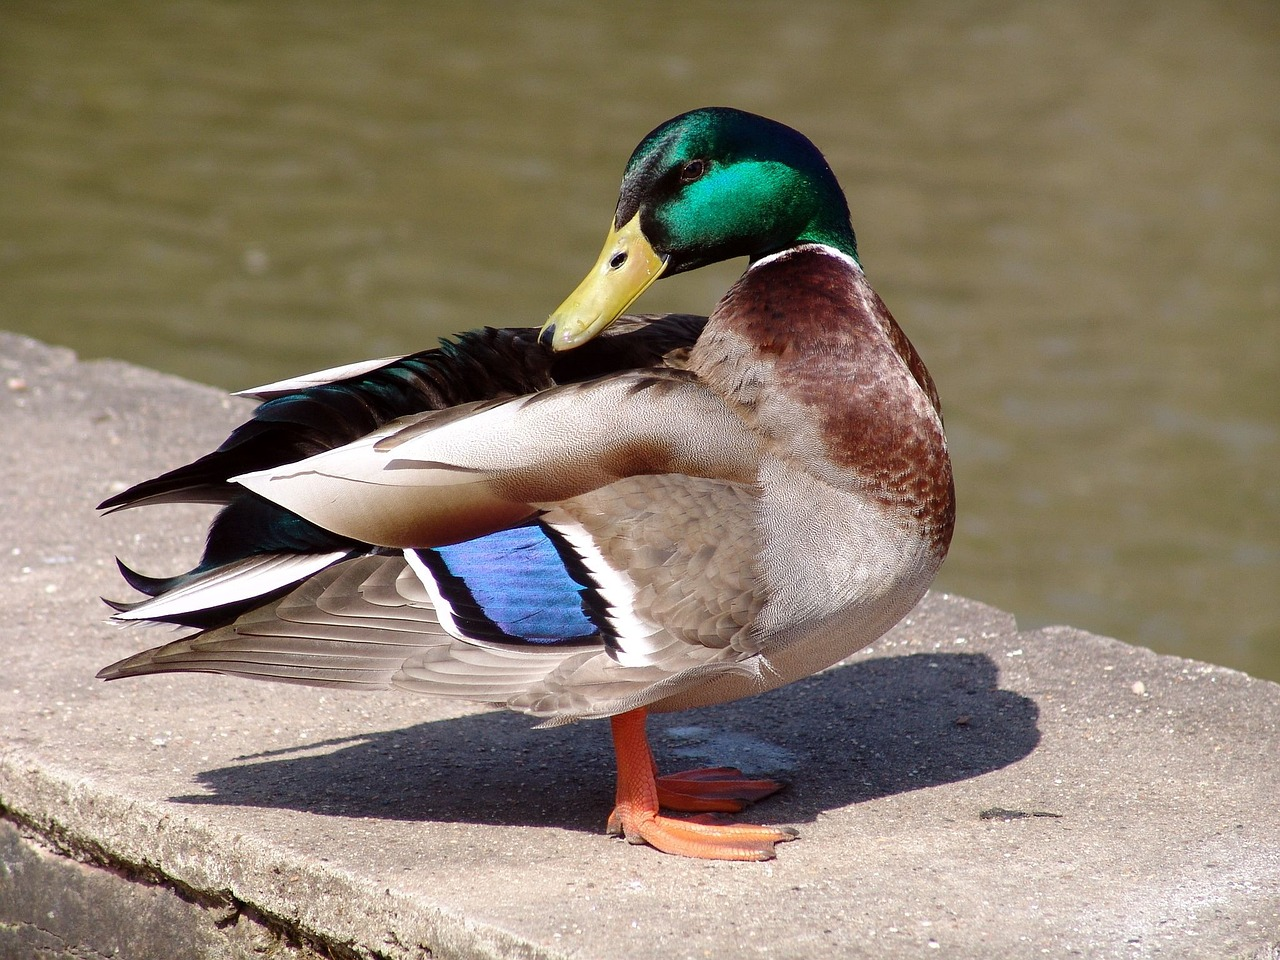
\includegraphics[width=\textwidth]{images/duck.jpg}


Da du aber wahrscheinlich ja eher Abbildungen machen willst versuche es hiermit.

\begin{figure}[h]
	\centering
	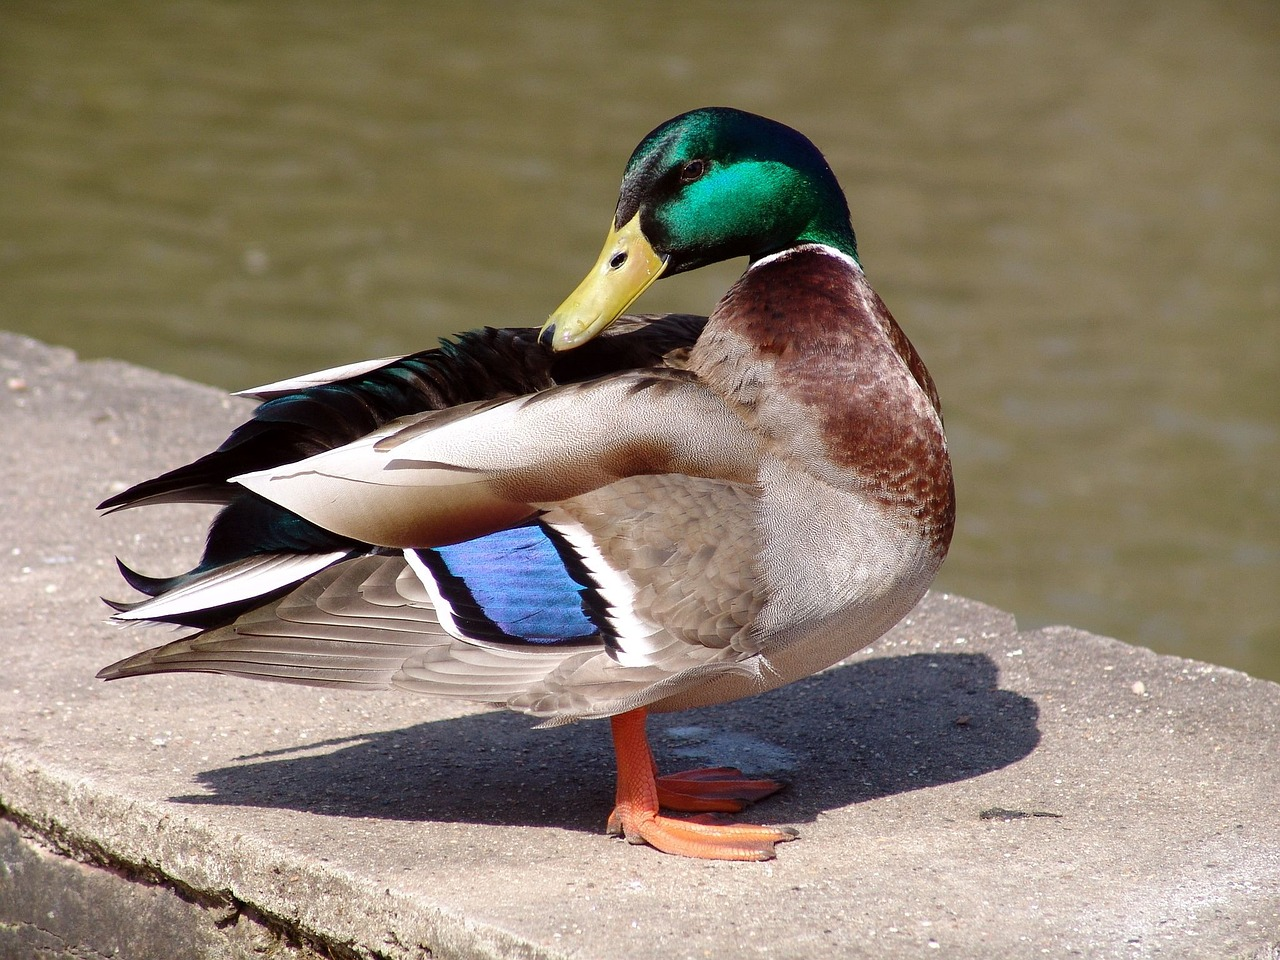
\includegraphics[width=0.7\textwidth]{images/duck.jpg}
	\caption{This is a smaller duck}
	\label{fig:duck}
\end{figure}